\documentclass[12pt,a4paper]{article}
\usepackage{geometry}
\geometry{left=2.5cm,right=2.5cm,top=2.0cm,bottom=2.5cm}
\usepackage{CJKutf8}
\usepackage[english]{babel}
\usepackage{amsmath,amsthm}
\usepackage{amsfonts}
\usepackage[longend,ruled,linesnumbered]{algorithm2e}
\usepackage{fancyhdr}
\usepackage{array}
\usepackage{listings}
\usepackage{color}
\usepackage{graphicx}
\graphicspath{ {./img/} }

\begin{document}
\begin{CJK*}{UTF8}{gbsn}

	\title{
		{\textbf《算法分析与设计》第 {$4$} 次作业
			\footnote{要求:1、分析题请用书面化语言给出详细分析过程。2、作业请统一使用hw0*-学号-姓名的命名格式,latex版本请附上源代码并打包提交。}
		}
	}
	\date{}

	\author{
		姓名:\underline{王骏}~~~~~~
		学号:\underline{71119138}~~~~~~
		成绩:\underline{~~~~~~~~~~~~~~~~~~}
	}

	\maketitle

	\noindent
	\section*{\bf \color{red}{算法分析题}}
	\noindent
	{\bf 题目1:}请按照提示用贪心算法设计一个的算法,该算法能用来确定有 $n$ 个整数的集合 $A[1..n]$ 中是否有两个数字之和正好等于一个给定的整数 $x$ 。并证明该算法时间复杂度为$\Theta(nlgn)$ 。\\
	提示:\\
	第一步,我们先将 $A[1..n]$ 排序。\\
	第二步,检查 $A[1] + A[n]$ 与 $x$ 的关系,分三种情况讨论。\\
	第三步,重复第二步的做法,在剩下的要检查的序列中把首尾两项相加,比较 $A[1] + A[n]$ 与 $x$ 的关系。

	\vspace{5pt}
	\noindent
	{\bf 答:}

	\begin{itemize}
		\item 算法:\\
			设i = 1,j = n;\\
			遍历i从1到n, 每次判断:
			$$
			\left\{ \begin{array}{lcl}
					A[i] + A[j] = x & \mbox{return} & true\\
					A[i] + A[j] < x & \mbox{do} & j = j + [\frac{n-j}{2}]\\
					A[i] + A[j] > x & \mbox{do} & j = j - [\frac{j-i}{2}] 
				\end{array}\right
				$$
			\item 复杂度证明:\\
				每个i对应的j的搜索为二分搜索,复杂度为logn\\
				i最坏遍历n次\\
				所以复杂度为\mathcal{O}(nlogn)
		\end{itemize}


		\vspace{10pt}
		\noindent
		{\bf 题目2:}某剧场举办一个电影节。剧场内有二个电影院,$X$ 和 $Y$ 。假设在从 $t = 0$ 开始的某一段时间内,电影院 $X$ 会顺序放映 $n$ 个长短不一的电影 $x_1$ ,$x_2$ ,…, $x_n$ 。其每场开始和结束时间顺序为 ($a_1$,$b_1$) , ($a_2$,$b_2$),…, ($a_n$,$b_n$)。从 $t = 0$ 开始,在同一期间,电影院 $Y$ 会连续放映 $m$ 个电影, $y_1$, $y_2$,…, $y_m$。 其每场开始和结束时间顺序为 ($c_1$,$d_1$), ($c_2$,$d_2$),…, ($c_m$,$d_m$)。我们规定每位观众必须准时入场并不得中途退场。假定两电影院之间距离极近,覌众从一个影院走到另一个所需时间为零。\\
		请根据提示设计一个贪心算法以决定同一个观众最多可以看完几场电影,并为他选出这些电影。你必须解释为什么你的算法可给出最佳的解,即保证看到最多的电影,并分析时间复杂度.\\
		提示:\\
		解的思路是,从 $t = 0$ 开始,决定下一场电影是去电影院 $X$ 还是 $Y$ 去看。如果 $b_1 \leq d_1$ 那么去电影院 $X$ 看 $x_1$。反之,如果 $b_1 > d_1$ 则选 $y_1$。一旦选中,那么下一个要做决定的时刻就是看完第一场电影那个时刻 ($b_1$ 或 $d_1$)。这时可用同样的原理来决定下一场电影是去电影院 $X$ 还是去 $Y$。
		\\	

		\vspace{5pt}
		\noindent
		{\bf 答:}

		\begin{itemize}
			\item 算法:

				将两个电影院的所有电影按结束时间的早晚排序后放入队列movie\_over\_queue中\\

				设置队列的第一个元素为第一场观看的电影,记为current\_movie\\
				current\_movie看完后,

				\begin{lstlisting}
while(current_movie.overTime > movie_over_queue.first.startTime)
{
	movie_over_queue.pop()
} 
current_movie <- movie_over_queue.first
movie_over_queue.pop()
				\end{lstlisting}

				遍历一遍队列

			\item 最优性证明:\\
				{\bf归纳基础:}证明存在的最优解A包含队列中第一项\\
				若A中第一个活动为j!=1,
				令$$A' = (A -{j})\cup{1}$$由于1的结束时间小于j的结束时间,所以A'也是最优解,且含1\\
				{\bf 归纳步骤:}
				假设命题对k为真,证明对k+1也为真\\
				执行到k步,选择了电影$1,i_2,i_3...i_k$\\
				由假设最优解A包含这些电影$i_1=1, i_2, i_3...i_k$,A中剩下活动选自集合
				$$S'=\{i|i \in S, s_i.overTime \geq i_k.overTime\}$$
				且
				$$
				A=\{i_1,i_2...i_k\}\cup B
				$$
				$B$一定是$S'$的最优解
				根据归纳基础,存在$S'$的最优解$B$含有$S'$中的第一个活动,设为$i_{k+1}$且
				$$|B'|=|B|$$
				于是
				$$\{i_1,i_2...i_k\} \cup B' = {i_1,i_2..i_k,i_k+1}\cup (B'-\{i_{k+1}\})$$
				也是原问题的最优解

		\end{itemize}

		\vspace{10pt}
		\noindent
		{\bf 题目3:}假设我们须要把 $n$ 个钢管,$a_1$, $a_2$, …, $a_n$ 焊成一根钢管。这些钢管的重量分别是$W[i]$, $1 \leq i \leq n$。每次焊接你可以从被焊钢管中任选二根来焊,但每次焊接的代价等于被焊两根钢管重量之和。比如我们有 $5$ 根钢管,重量为 $3$, $8$, $5$, $10$,$13$。显然,任何一个焊接计划可以用一个有 $n$ 个叶子的完全二义树表示。如果我们按下面二叉树所示的顺序焊接,那么总的代价为 $(5+8) + (13+13) + (3+10) + (26+13) = 91$. \\
		\begin{figure}[h]
			\centering %图片居中
			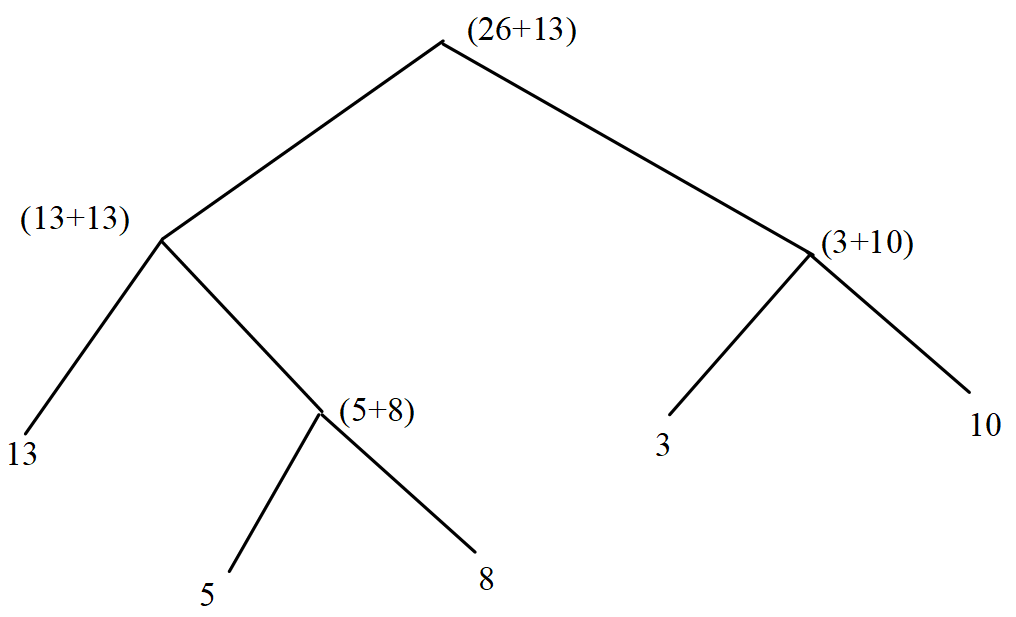
\includegraphics[width=0.7\textwidth]{1} %插入图片,[]中设置图片大小,{}中是图片文件名
		\end{figure}

		\begin{enumerate}
			\item[(a)]  假设有一个 $n$ 个叶子的完全二叉树 $T$ 表示一个焊接计划,证明这个焊接计划的总代价为 $Cost(T)=\sum_{k=1}^{n} W[k]depth(k)$,其中$depth(k)$是代表钢管 $a_k$ 的叶子在树中的深度。
			\item[(b)]  如果一个焊接计划有最小的总代价,则称为最佳焊接计划。证明在一个代表最佳焊接计划的二叉树 $T$ 中,代表最轻二根钢管的叶子在最底层。
			\item[(c)]  证明有一个最佳焊接计划,它的第一步是把最轻的二根钢管焊在一起。
			\item[(b)]  设计一个有效算法为这 $n$ 个钢管产生一个最佳焊接计划。
		\end{enumerate}

		\vspace{5pt}
		\noindent
		{\bf 答:}

		\begin{itemize}
			\item{a}
				由于每个叶子节点到根的过程即为焊接的过程,所以每上一层,需焊接一次,故每个叶子节点共需代价为$$W[k]depth(k)$$累加起来得总代价
				$$\sum_{k=1}^{n} W[k]depth(k)$$

			\item{b} {\bf 反证}假设有个最佳计划的最轻的两个管子不在最底层,则我们将在最底层的情况中最轻的两个管子与这个最佳计划的占据相同位置的两个管子进行交换,假设管子重量$W[k]$已按从轻到重排序


				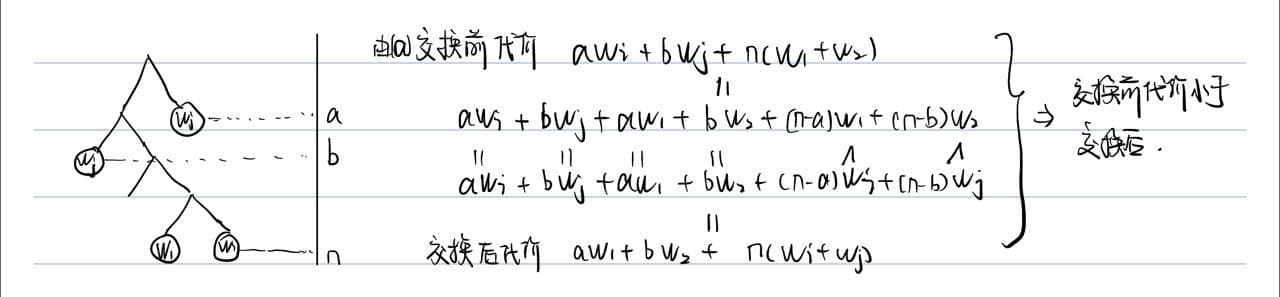
\includegraphics[width=15cm]{img/answ3.jpg}

				故这个最佳计划没有最轻的两个管子在最底层的优

			\item{c} 假设有个计划第一步不将最轻的两个旱在一起,我们将最轻的两个与这两个交换位置,由(b)最轻的两个一定在最底层,故交换后由(a)可知,代价没变,所以这个计划也是最优的,故一定存在一个最优计划第一步是把这两个最轻的焊接在一起
			\item{d} {\bf 即哈夫曼树的生成方法}

				1. 将这些管子按轻重放入队列,每次将队列的前两个焊接起来形成一个新的节点,这两个出队列\\
				2. 在将新的节点入队列合适位置重复1的操作

		\end{itemize}


	\end{CJK*}
	\end{document} 
